\chapter{基于应用场景的系统层能效优化}

本章首先介绍了动态电压频率调节(DVFS)的基本概念以及其在能效优化领域所发挥的作用。本章利用前述章节所实现的CNN运行时库开发了一款智能监控系统Android应用。\ref{chapter5-2}节对该应用的负载特征进行了刻画与分析,阐述了当前Android系统所采用的功耗管理器在基于深度学习模型应用上表现的不足之处。\ref{chapter5-3}节提出了一种基于应用场景的系统层能效优化策略,该策略根据应用在系统层表现的负载特征对其进行分类,这样系统便可以针对不同的应用使用不同的功耗管理策略。

\section{动态电压频率调节技术}

动态电压频率调节(Dynamic Voltage and Frequency Scaling, DVFS)是一种可对芯片电压和频率进行实时动态调节的技术。当前手机CPU和GPU都支持DVFS,并且系统层也都存在着相应的功耗管理器(governor)。每一个功耗管理器都拥有一个执行频率调节的策略,并且这个策略可被配置以取得不同的能效折中。根据配置的策略,功耗管理器可以决定不同状态下的设备处理器所应该运行的频率。设备处理器的负载越高运行频率越高是这些功耗管理器所遵循的基本准则。

动态功耗\cite{benini1999policy}、短路功耗\cite{周宽久2010嵌入式软硬件低功耗优化研究综述倡}和漏电流功耗\cite{you2006compilers}是CMOS电路的三个主要功耗,因此CMOS电路的总功耗可由公式\ref{equation:equation3}表示:

\begin{equation}
     \label{equation:equation3}
     \begin{aligned}
        P = P_{Dynamic} + P_{Short} + P_{Leakage}
         = ACV^2f +  AVI_{Short} + VI_{Leakage}
     \end{aligned}
\end{equation}

式中$C$代表负载电容的容值,$V$是工作电压,$A$是当前频率下电路的平均翻转率,$f$为工作频率,$I_{Short}$和$I_{Leakage}$分别为短路电流和漏电流。从公式中可知,$C$、$V$、$A$、$f$决定了整个CMOS电路的功耗,而DVFS技术就是主要通过改变频率$f$和电压$V$的值来调节系统功耗的。


\section{智能监控系统Android应用的负载分析}
\label{chapter5-2}

基于前述章节所实现的CNN运行时库,本文开发了一款智能监控系统Android应用,其可以通过手机摄像头自动辨识周围所观察到的物体类别。图\ref{figure:figure31}显示了两张该应用的运行界面。智能监控系统应用的智能识别功能是由卷积神经网络Tiny YOLO\cite{pjreddie.com}卷积模型提供的。

\begin{figure}[htbp]
    \centering
    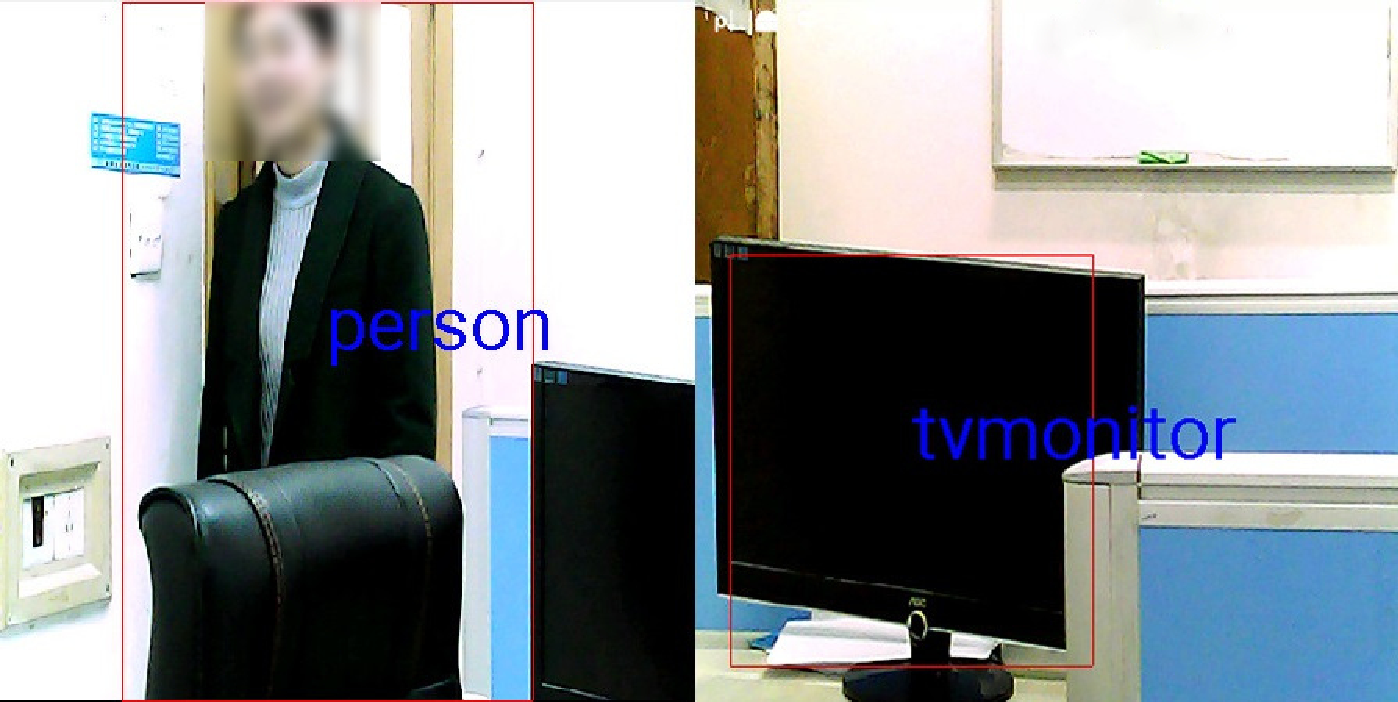
\includegraphics[height=0.4\textwidth]{figures/app.pdf}
    \caption{智能监控系统Android应用}\label{figure:figure31}
\end{figure}

图\ref{figure:figure36}显示了智能监控系统Android应用的工作流程。在智能监控系统APP启动后,它会不断地通过手机摄像头感知周围的场景。当读取到摄像头所拍摄视频中的一帧数据后,该APP会立即将该帧数据作为CNN模型的输入并执行网络的前向推断过程。推断完成后,侦测结果会在视频框中显示出来。紧接着,监控APP会立即获取下一帧图像数据并重复上述过程。

\begin{figure}[htbp]
    \centering
    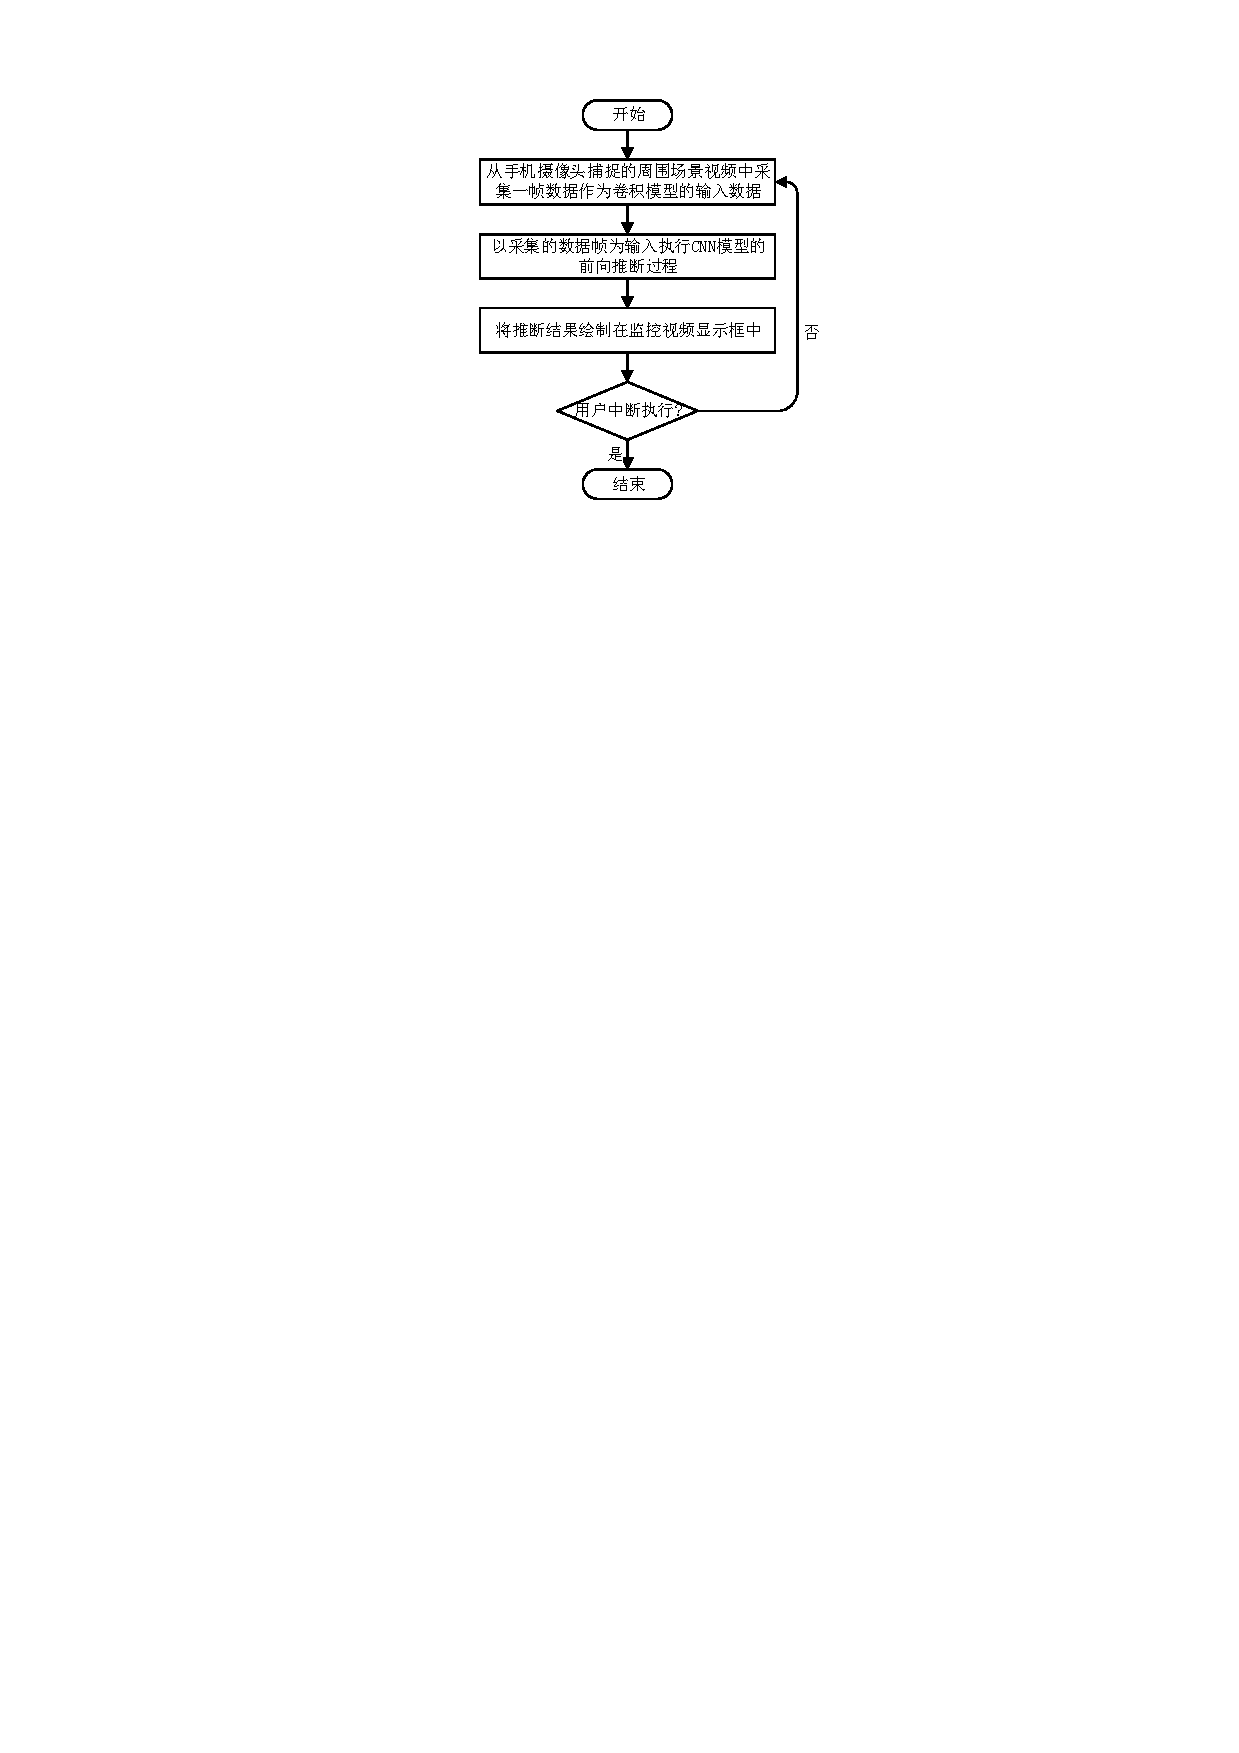
\includegraphics[height=0.5\textwidth]{figures/app_process.pdf}
    \caption{智能监控系统APP的工作流程}\label{figure:figure36}
\end{figure}

为了探索从系统层进一步优化基于CNN模型的手机应用,本文基于ODROID-XU3平台考察了智能监控系统APP的运行时负载特征。由第\ref{chapter:chapter4}章可知,智能监控系统APP在ODROID-XU3上主要使用GPU执行CNN的前向推断过程,故而可使用GPU的利用率作为该APP的负载。图\ref{figure:figure37}显示了在Android系统GPU默认功耗管理策略下智能监控系统APP的负载和GPU频率变化情况。

由图\ref{figure:figure37}的GPU利用率曲线可以看出,智能监控系统APP的负载(GPU利用率)平均值为86.59\%,并且绝大多数的负载值都在平均线以上。智能监控系统APP的负载曲线形状类似了周期脉冲图,这与该APP的实际工作流程相符合。因为智能监控系统APP的工作流程就是周期性的“采样-推断-绘制”。由智能监控系统APP的负载曲线上只有一个很窄的波谷可知,“采样-推断-绘制”三个操作中推断占了整个APP运行周期的绝大部分。

\begin{figure}[htbp]
    \centering
    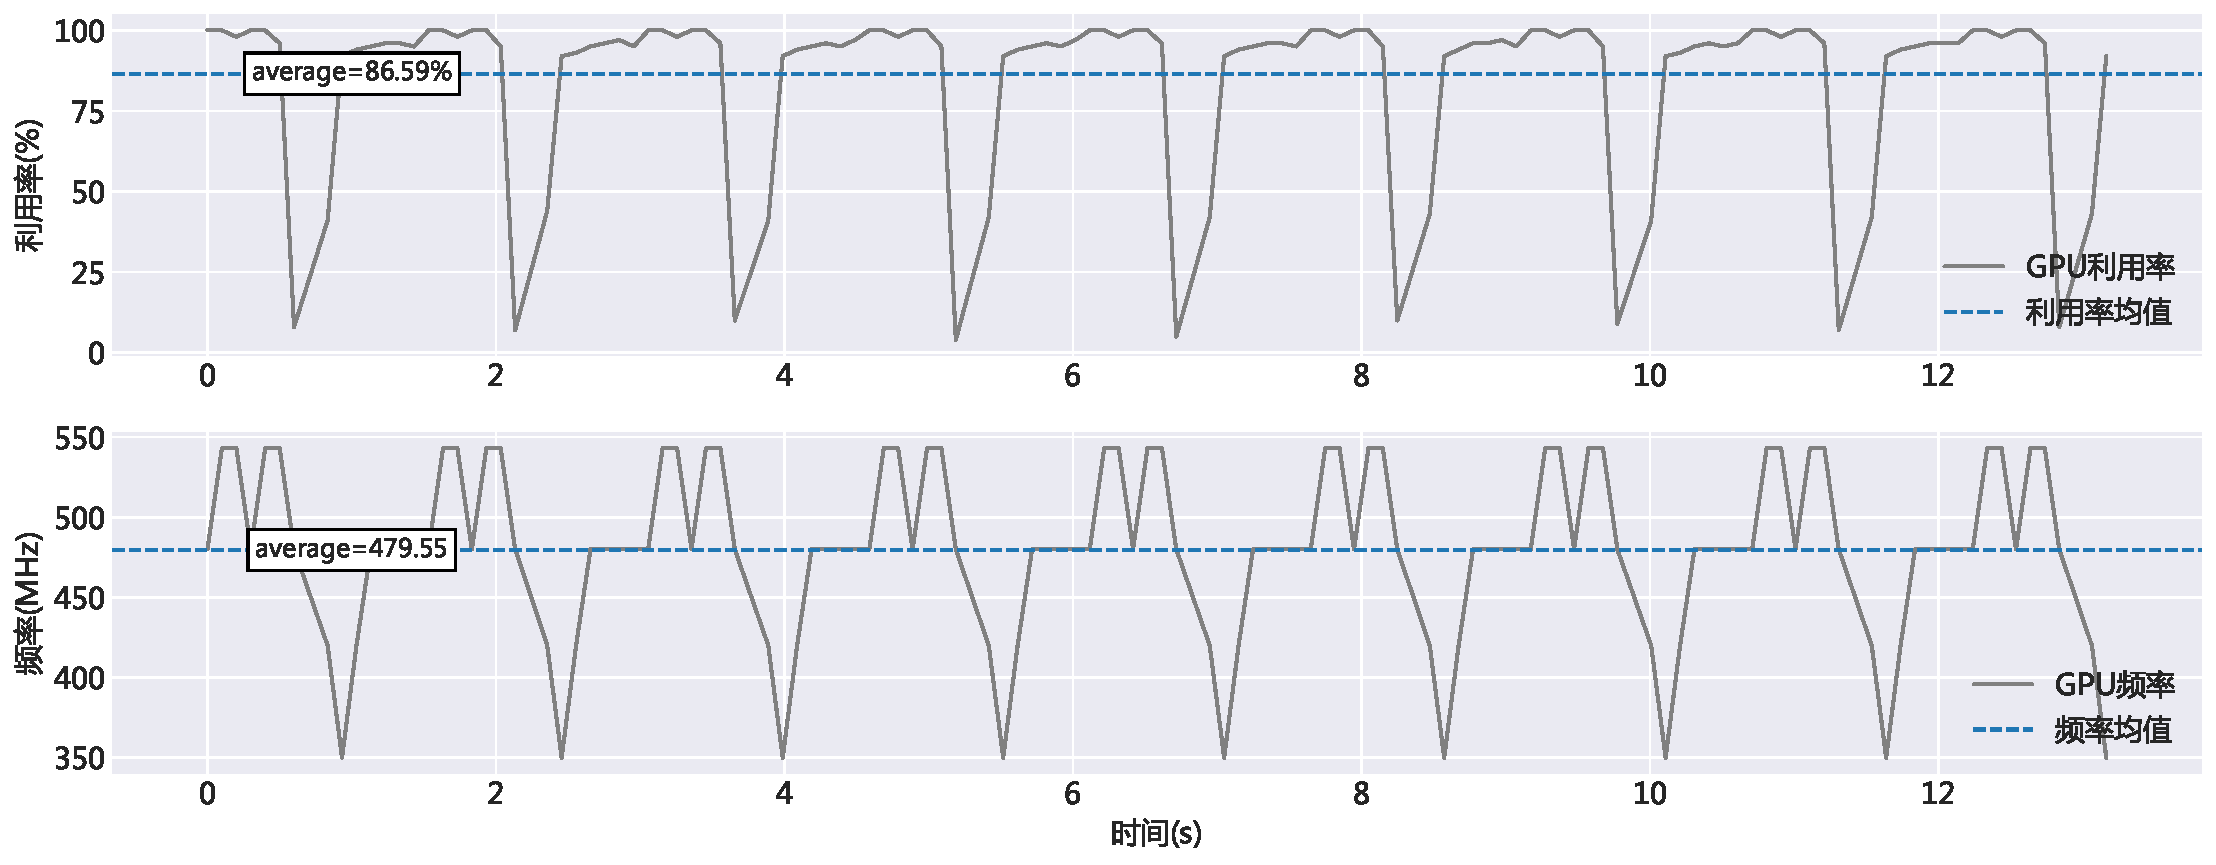
\includegraphics[width=1.0\textwidth]{figures/system_util.pdf}
    \caption{智能监控系统APP的负载和GPU频率变化}\label{figure:figure37}
\end{figure}

图\ref{figure:figure37}的GPU频率曲线即反映了GPU默认功耗管理器所采用的调频策略针对智能监控系统APP负载所进行的频率调节变化。由于智能监控系统APP负载存在一个尖脉冲波谷,所以在默认调频策略下GPU的频率不断在350MHz至543MHz之间抖动(均值约为480MHz)。另外,由于频率是根据负载的变化进行调整的,所调频具有一定的迟滞性。从图\ref{figure:figure37}中两条曲线的变化可以明显看出,当负载处于较低位置时,频率仍在较高点;当GPU几乎处于满负载的状态下,频率却在480MHz与543MHz间跳变,产生“乒乓效应”。频率调节的迟滞性会造成不必要的功耗开销,而“乒乓效应”不仅带来额外的调频开销还会导致上层应用的性能损失。

ODROID-XU3平台所配备的\texttt{Mali-T628 MP6} GPU支持六级调频,即GPU的运行频率可设置为177MHz,266MHz,350MHz,420MHz,480MHz和543MHz六个值。本文将GPU频率分别保持在这六个频率值上,考察了智能监控系统APP中一次CNN推断的运行时间、能耗和功耗的变化情况,结果如图\ref{figure:figure38}所示。从图中三条曲线的走势可以看出,随着GPU运行频率的提高,CNN推断的运行时间在不断减小,而GPU的功耗和能耗在逐渐上升。图\ref{figure:figure38}中的能耗曲线在266MHz处上升幅度较大,并且从功耗曲线中也可以发现266MHz和350MHz处的GPU功耗相同,这可能是因为\texttt{Mali-T628 MP6} GPU在266MHz的运行时功耗没有优化好。

图\ref{figure:figure38}中的虚线标注出了在GPU默认功耗管理策略下APP中CNN推断的运行时间、能耗和功耗,从中可以发现GPU保持运行在480MHz时的运行时间、能耗及功耗与默认功耗管理策略下的对应值十分相近。由图\ref{figure:figure37}可知,默认功耗管理策略下执行CNN推断时GPU频率均值约为480MHz,这也解释了前述两者在性能和功耗上表现相似的原因。

\begin{figure}[htbp]
    \centering
    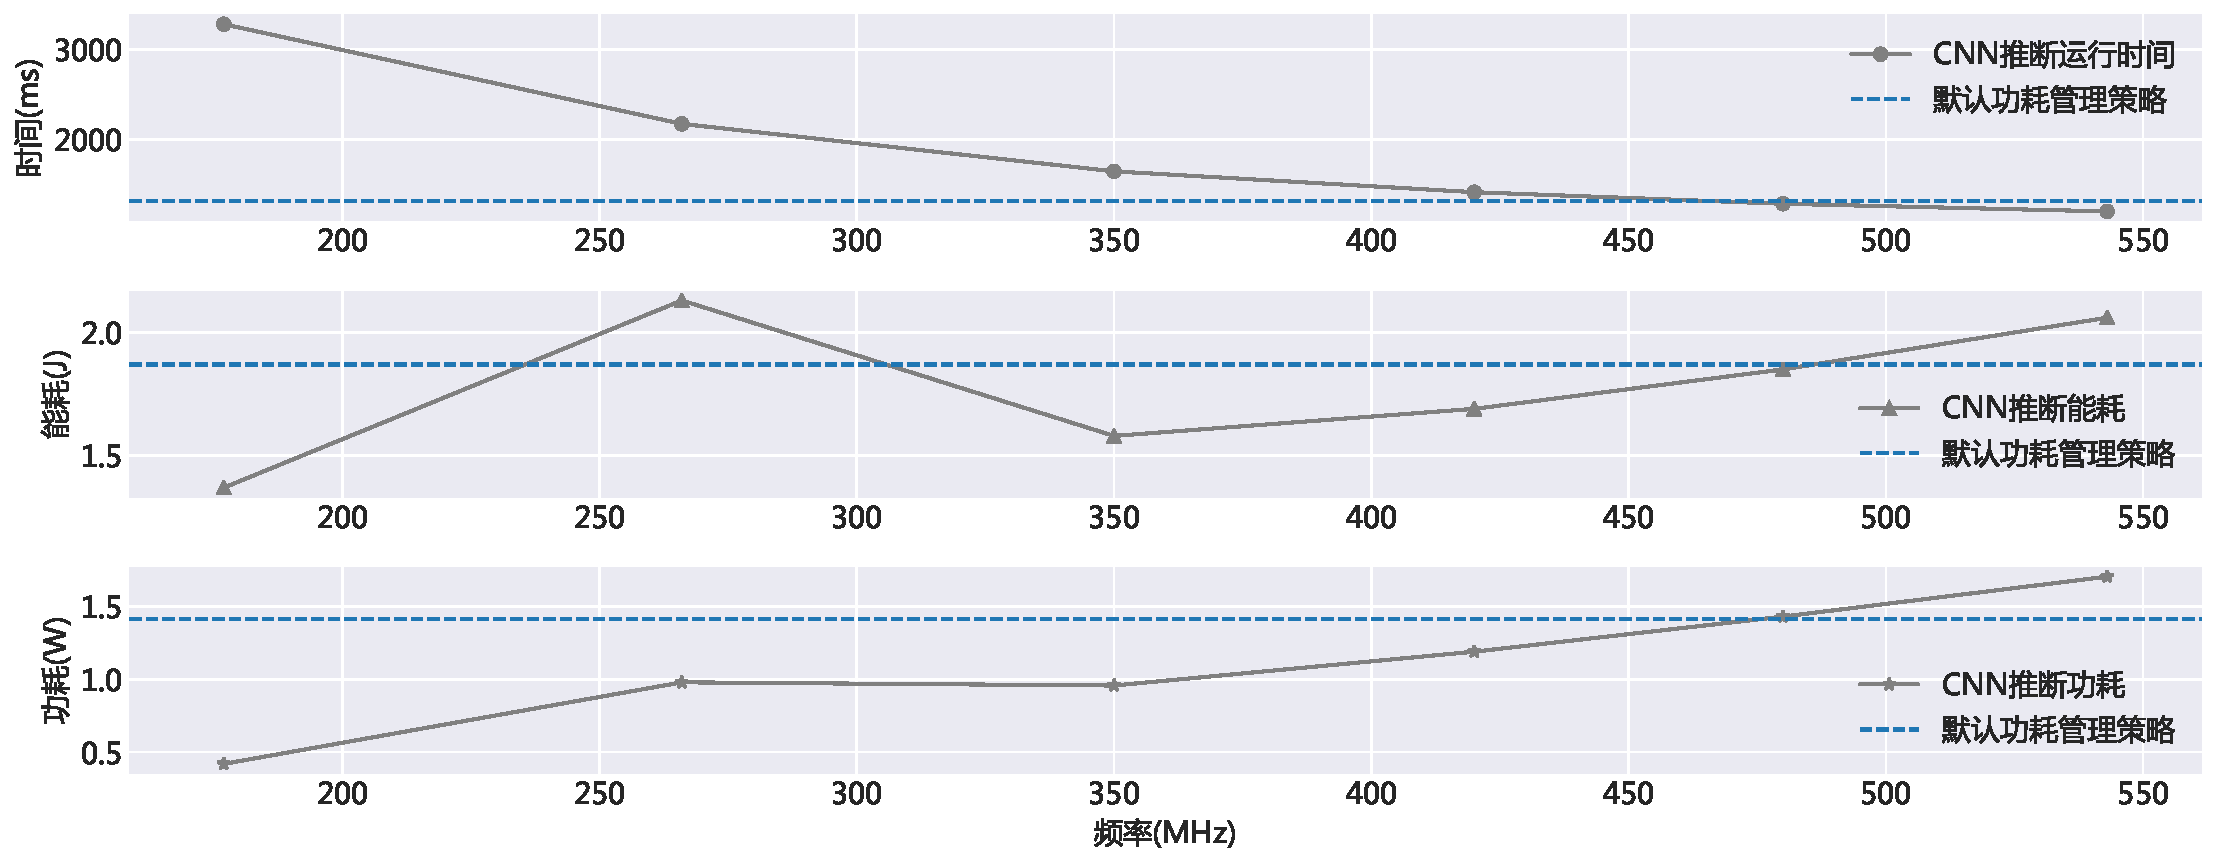
\includegraphics[width=1.0\textwidth]{figures/system_explore.pdf}
    \caption{CNN推断的运行时间、能耗和功耗随GPU频率的变化}\label{figure:figure38}
\end{figure}

表\ref{table:table11}进一步分析比较了GPU默认功耗管理策略与GPU保持在某一固定频率时执行CNN推断的能效。本文使用\texttt{FPS}(每秒处理图像数据的帧数)作为性能指标,并且使用EDP值评估不同策略的能效。表中的性能提升、能耗和功耗降低数据都是相对于默认调频策略而言的。

\begin{table}[htbp]
  \centering
  \caption{智能监控系统APP在不同调频策略下的能效}
  \label{table:table11}
\resizebox{1.0\textwidth}{!}{
  \begin{tabular}{ccccccccc}
    \toprule
      策略 & 运行时间(ms) & 性能(FPS) & 能耗(J) & 功耗(W) & EDP(Joules*seconds) & 性能提升 & 能耗降低 & 功耗降低\\
    \midrule
    默认调频策略 & 1323.83 & 0.76 & 1.87 & 1.41 & 2.48 & — & — & — \\
    固定最低频率 & 3277.89 & 0.31 & 1.37 & 0.42 & 4.49 & -59.61\% & 26.74\% & 70.41\% \\
    固定最高频率 & 1207.85 & 0.83 & 2.06 & 1.71 & 2.49 & 9.60\%	& -10.16\% & -20.74\% \\
    固定480MHz  &  1292.83 & 0.77 & 1.85 & 1.43 & 2.39 & 2.40\% & 1.07\% & -1.30\% \\
    \bottomrule
  \end{tabular}
}
\end{table}

由表\ref{table:table11}可以看出,将GPU频率固定到480MHz时,智能监控系统APP的执行性能不仅有所提升而且其能耗也有所降低,这就证明了调频迟滞性和“乒乓效应”确实会造成不必要的能耗开销和性能损失。分析各种策略的EDP值可知,GPU频率固定在最低频率时能效最低,而使用默认调频策略、固定480MHz以及固定最高频率时能效相近。虽然固定GPU运行在480MHz时,EDP能效值最低,但是与默认调频策略相比其在性能上的提升量(1.07\%)和功耗上的降低量(2.40\%)均不太明显。而固定GPU运行在最高频率与默认调频策略的能效EDP值几乎一样,但是其在性能上会带来约9.8\%的提升。综上所述,对于内嵌CNN模型的智能监控系统APP而言,直接将GPU频率调至最高点比使用默认GPU调频策略更佳。

\section{基于应用场景的系统层能效优化策略}
\label{chapter5-3}

经过第\ref{chapter5-2}章节的分析可知,针对基于CNN模型的生活日志型Android应用(如本文开发的智能监控系统APP),系统默认使用的调频策略会产生“乒乓效应”并造成额外的能耗开销,而将GPU频率固定在最大可达频率处CNN推断性能更高且几乎不影响推断的能效。因此,本文提出基于应用场景的调频策略,其可自动感知系统上层运行的应用类别。具体来说,若该策略感知到系统上层运行的是基于CNN模型的生活日志型Android应用,其会将GPU频率调至最高点并保持不变;若该策略感知到系统上层运行的是传统型应用,其会使用GPU原默认的调频策略。基于应用场景的调频策略主要根据系统上层应用的负载特征对应用进行分类,并在分类过程中使用动态时间规整计算上层应用所属的类别。

\subsection{动态时间规整}
\label{chapter5-3-1}
在时间序列分析领域,动态时间规整(Dynamic Time Warping,DTW\cite{muller2007dynamic})主要用于衡量两段时间序列的相似度,并且这两段时间序列的变化速度可以是不一致的。例如,语音识别中不同人的语速不同,同一个字母的发音序列会有所差别,但使用DTW就可以有效的区分这种同字母不同语速下的语音序列。动态时间规整主要通过将两段时间序列进行延伸和缩短来计算它们之间的相似性。如图\ref{figure:figure39}所示,序列X和序列Y表示两段时间序列,双箭头指向处代表两段序列间的对齐点。

\begin{figure}[htbp]
    \centering
    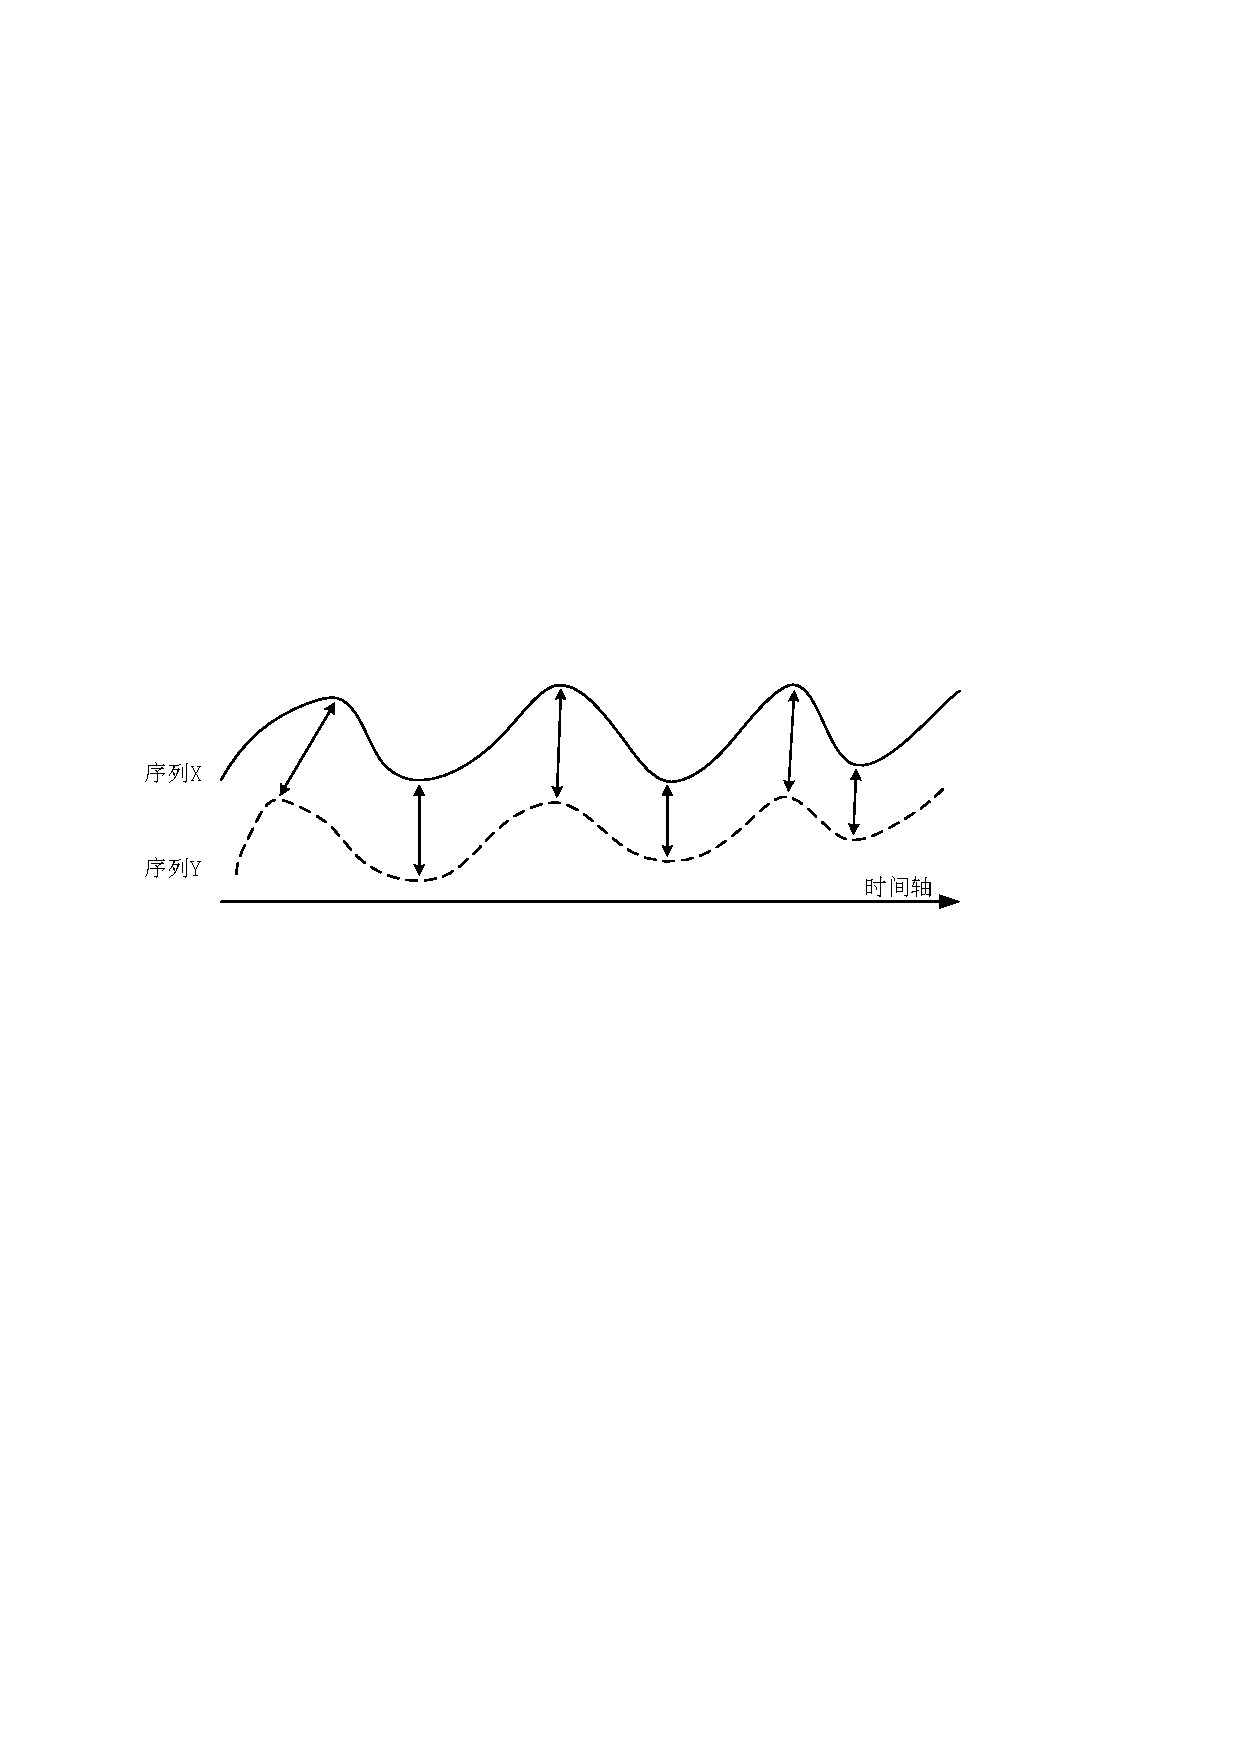
\includegraphics[width=0.8\textwidth]{figures/dtw.pdf}
    \caption{两段时间序列间的规整}\label{figure:figure39}
\end{figure}

\begin{equation}
    \label{equation:equation4}
    \begin{aligned}
        D(i,j) = d(i,j) + min{D(i-1,j),D(i,j-1),D(i-1,j-1)}
    \end{aligned}
\end{equation}

图\ref{figure:figure40}展示了求取两段时间序列间DTW值的一个示例,其中DTW的主要计算步骤如下所述:
\begin{enumerate}
  \item 计算两段时间序列各对齐点间的距离$d(i,j)$,这里可以使用欧氏距离、曼哈顿距离等。
  \item 设置$i = 0$和$j = 0$处的规整距离$D(i,j)$为正无穷大。
  \item 对于$i = 1 ... n$,$j = 1 ... m$,利用公式\ref{equation:equation4}迭代计算各个对齐点间的规整距离$D(i,j)$。
  \item 最后一次迭代结果$D(n,m)$即为所求两时间序列间的动态时间规整距离。
\end{enumerate}

\begin{figure}[htbp]
    \centering
    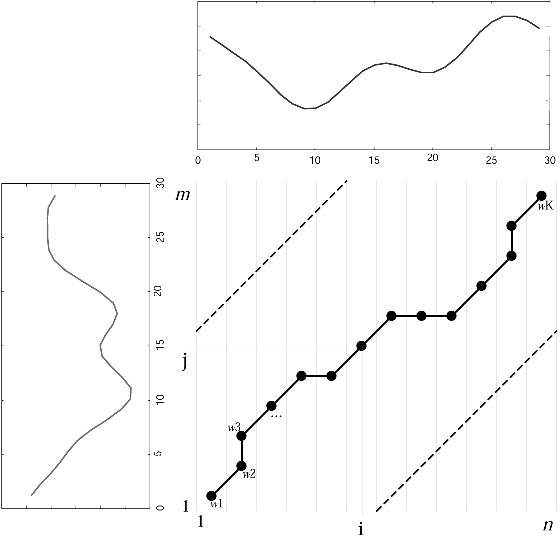
\includegraphics[height=0.56\textwidth, width=0.65\textwidth]{figures/dtw_dist.pdf}
    \caption{规整路径示例 \cite{keogh2001derivative}}\label{figure:figure40}
\end{figure}

\subsection{基于应用场景的调频策略}

如前所述,手机端内嵌CNN模型的生活日志型应用主要使用GPU执行推断过程,所以本文针对GPU设备处理器提出了基于应用场景的调频策略。算法\ref{algo:algorithm10}给出了本文所提策略的伪代码,其核心思想描述如下:
\begin{enumerate}
  \item 提取基于CNN模型生活日志型应用的特征负载时间序列$X(x_0, x_1, ... , x_ {N-1})$作为模板序列。
  \item 确定可对应用场景进行分类的DTW阈值$DTW_{TH}$,其可用于识别系统上层所运行应用是否为基于CNN模型的生活日志型应用。
  \item 每次进入调频函数,在长度为M的数组load\_infos中记录当前获得的负载值,并使计数器值加1。注意,M取值应使数组load\_infos能够覆盖上层应用的负载特征,其可由用户输入也可取一个较大值。
  \item 当计数器值等于M-1时,计算已获取的M个历史负载序列load\_infos和模板序列X之间的DTW值dtw\_dist。
  \item 当dtw\_dist小于$DTW_{TH}$时,说明系统上层所运行应用为基于CNN模型的生活日志型应用,此时应将GPU频率设置到最高(已最高则不变);反之,说明系统上层所运行应用为非基于CNN模型的其他应用,此时应采用GPU默认的调频策略。
\end{enumerate}

\begin{algorithm}[htbp]
  \small
  \SetAlgoLined
    \KwData{基于CNN模型的生活日志型应用负载模板序列$X(x_0, x_1, ... , x_ {N-1})$\;应用场景分类DTW阈值$DTW_{TH}$。}
    令函数dtw(X,Y)的功能为计算两段时间序列X和Y间的DTW值\;
    \textbf{初始化}count = 0;//计数已获取的负载值数量,仅全局初始化一次 \\
    \textbf{初始化}load\_infos[M] = {0};//存储最近获取的M个负载值,仅全局初始化一次 \\
    \textbf{初始化}dtw\_dist = 2$DTW_{TH}$; //仅全局初始化一次 \\
    \eIf{$count < M-1$}{
        load\_infos[count] = 当前GPU利用率(即上层应用负载)\;
        count++\;
    }{
        load\_infos[count] = 当前GPU利用率(即上层应用负载)\;
        count = 0\;
        dtw\_dist = dtw(X,load\_infos)\;
    }

    \eIf{$dtw\_dist < DTW_{TH}$}{
        将GPU频率调至最高一级,已最高则不变;//基于CNN模型的生活日志型应用 \\
    }{
        使用默认调频策略; //非基于CNN模型的其他应用
    }
  \caption{基于应用场景的调频策略}
  \label{algo:algorithm10}
\end{algorithm}

\section{实验验证}

本文利用ODROID-XU3平台实现了基于应用场景的调频策略,并使用所开发的智能监控系统Android应用对所提调频策略的有效性进行了验证。

根据图\ref{figure:figure37}显示的智能监控系统Android应用的负载(GPU利用率)曲线可知,包含完整CNN推断的负载序列时间长度小于2秒。因此,本文使用时间长度约为4秒的负载序列作为基于CNN模型的生活日志型应用负载模板序列,该序列总共包括40个负载值。为了确定可对不同应用场景进行分类的DTW阈值,本文分别考察了包括CNN推断在内的手机系统可能存在的几个应用场景下应用负载序列与模板序列间的DTW值,结果如图\ref{figure:figure41}所示。根据图\ref{figure:figure41}显示的结果可知,当DTW阈值取480时,基于CNN模型的生活日志型应用和非基于CNN模型的其他应用可以被很好地区分开来。实验中,针对智能监控系统Android应用,调频策略中的M参数只要取大于20的数字即可覆盖监控系统APP的负载特征。

\begin{figure}[htbp]
    \centering
    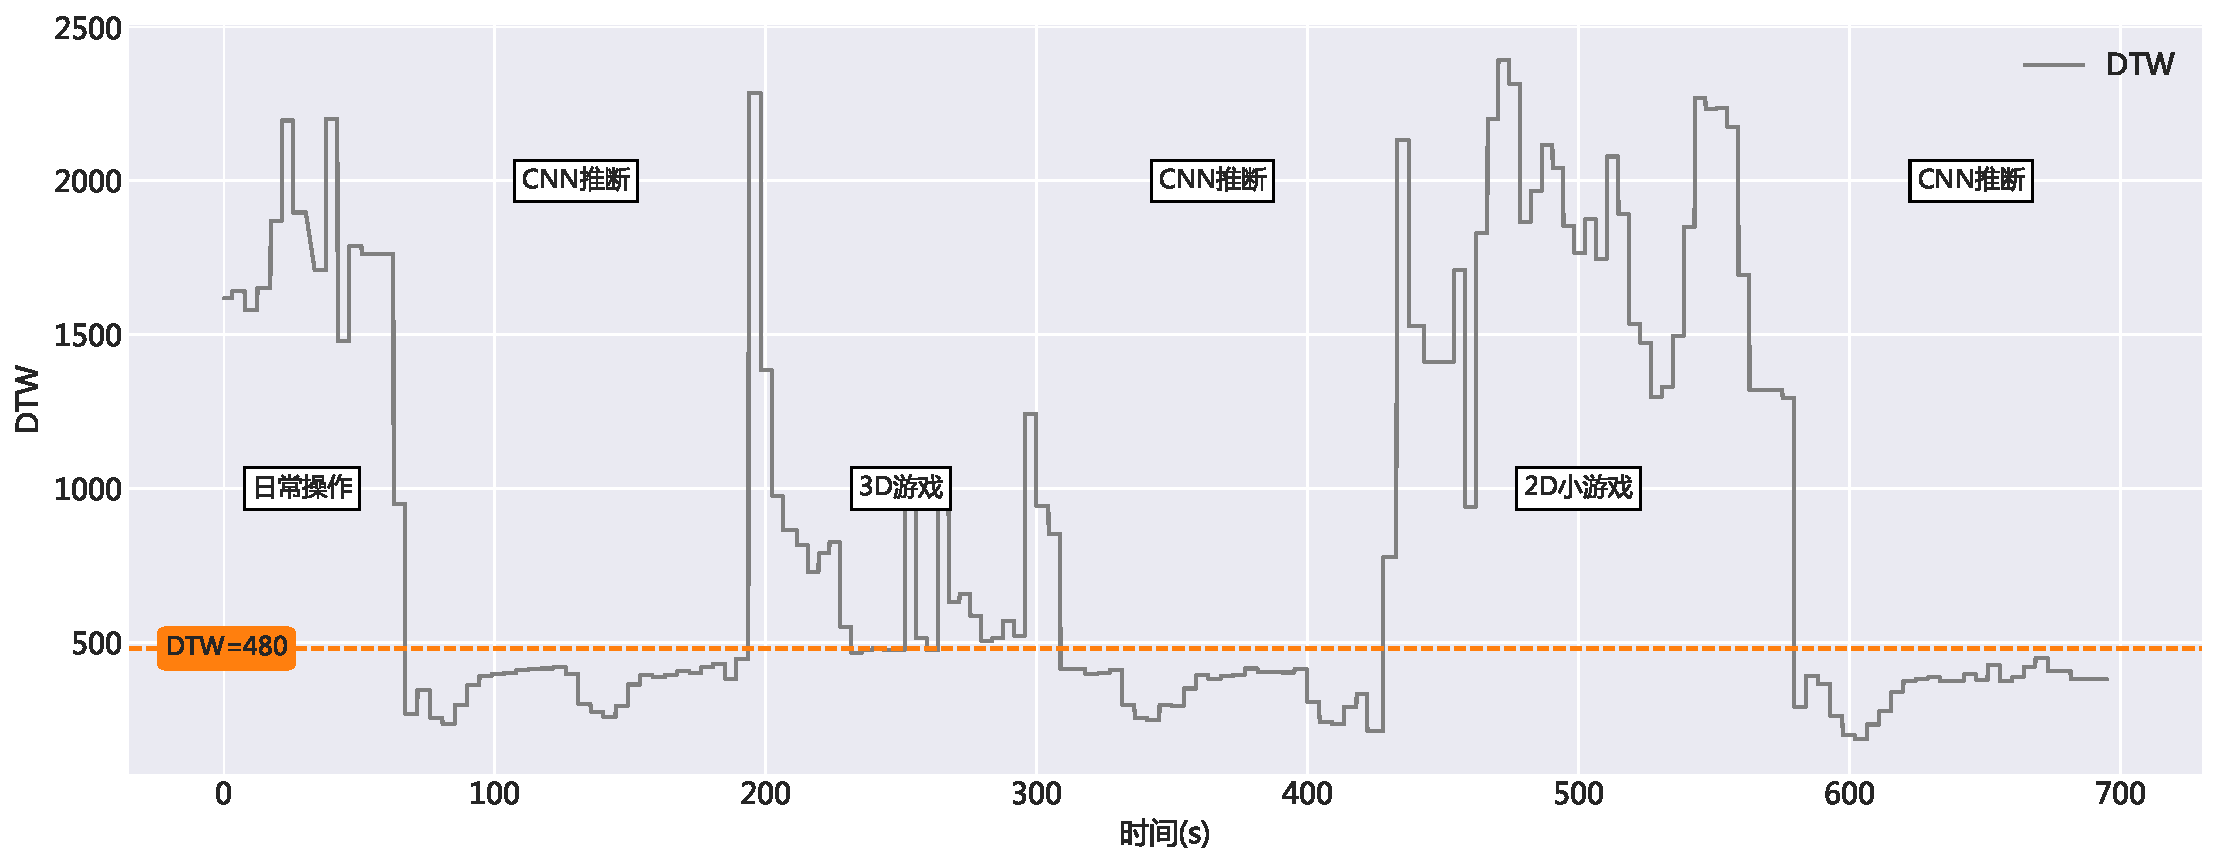
\includegraphics[width=1.0\textwidth]{figures/system_dtw.pdf}
    \caption{应用场景分类DTW阈值的确定}\label{figure:figure41}
\end{figure}

图\ref{figure:figure42}显示了基于应用场景的调频策略运行效果。由GPU的频率变化曲线可以看出,在手机系统处于日常操作(如查看邮件、联系人等)、3D游戏、2D游戏等应用场景下时,系统GPU功耗管理器使用的均为默认策略,而一旦系统检测到上层运行的应用为基于CNN模型的生活日志型应用时,很快会将GPU频率调至最高点并保持运行在最高频率。

\begin{figure}[htbp]
    \centering
    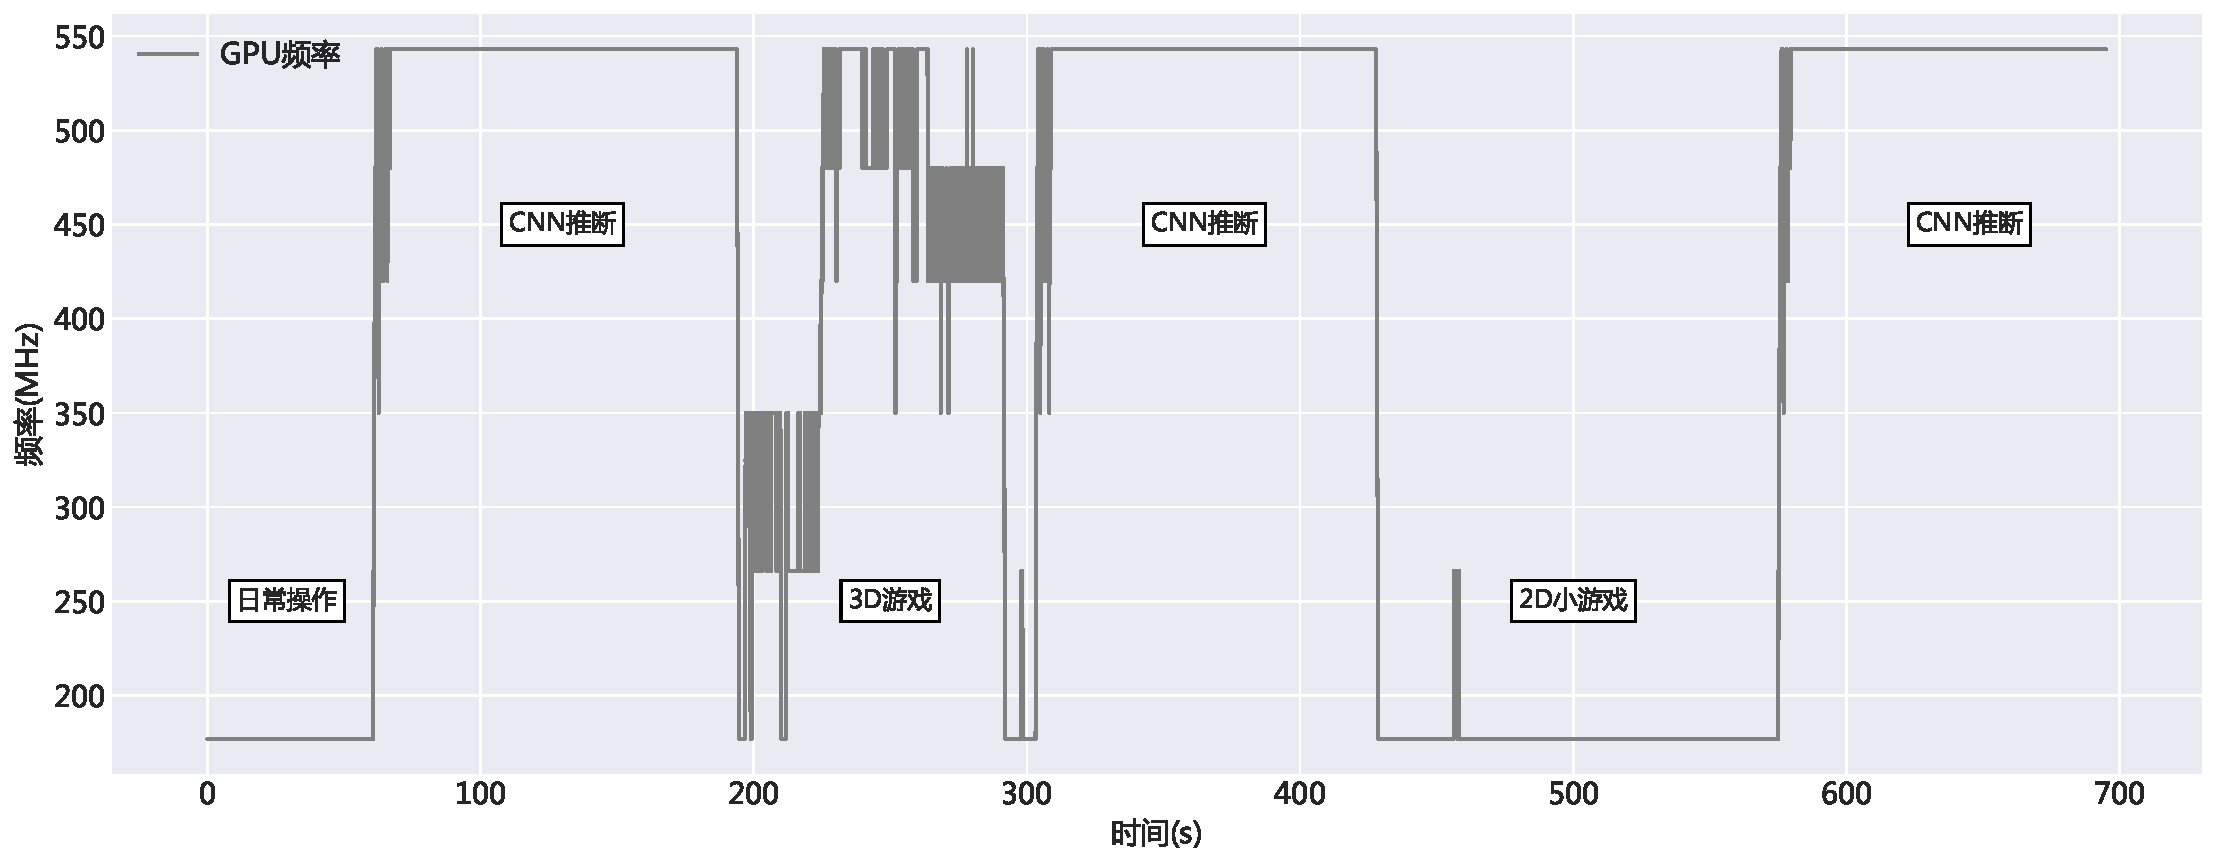
\includegraphics[width=1.0\textwidth]{figures/system_governor.pdf}
    \caption{基于应用场景的调频策略运行效果}\label{figure:figure42}
\end{figure}

为了分析基于应用场景的调频策略对系统功耗的影响,本文比较了分别于所提调频策略和默认调频策略下运行CNN推断时系统CPU功耗的变化。之所以仅比较CPU功耗,是因为系统功耗管理器都是运行在CPU上的。由表\ref{table:table12}可以看出,在默认调频策略和本文所提调频策略下,运行CNN推断时CPU的功耗分别为0.71W和0.72W。由此得出结论:在功耗测量误差范围内,基于应用场景的调频策略对系统功耗的影响可以忽略不计。

\begin{table}[htbp]
  \centering
  \caption{CNN推断过程中不同调频策略下CPU的功耗}
  \label{table:table12}
  \begin{tabular}{cc}
    \toprule
      策略 & CPU功耗(W) \\
    \midrule
      默认调频策略 & 0.71 \\
      基于应用场景的调频策略 & 0.72 \\
    \bottomrule
  \end{tabular}
\end{table}

\section{本章小结}
本章利用前述章节所实现的CNN推断时库开发了一款智能监控系统Android应用,并针对该应用详细分析了其在系统层所表现的负载特征。通过对比分析智能监控系统应用分别于GPU默认调频策略和固定频率策略下运行时的性能和能效,本文发现系统默认使用的调频策略会产生“乒乓效应”并造成额外的能耗开销,而将GPU频率固定在最大可达频率处CNN推断性能更高且几乎不影响推断的能效。因此,本的最后提出了一种基于应用场景的调频策略,其可自动感知系统上层运行的应用是否为基于CNN模型的生活日志型应用,并根据检测结果及时改变调频行为。

\cleardoublepage 